% !TeX spellcheck = en_GB
\begin{figure}
  \setlength{\unitlength}{\textwidth}
  \begin{picture}(1,0.3)(-0.02,0)
          
    \put(0.048,0.04){\includegraphics[width=0.45\unitlength]{./chapter-pi_1_pi_2/FnP/gnuplot/p_max.eps}}
    \put(0.54,0.04){\includegraphics[width=0.45\unitlength]{./chapter-pi_1_pi_2/FnP/gnuplot/p_2_p_max.eps}}
        
    \put(0.48,0.07){ \rotatebox{90}{$\displaystyle\massdamp$ \scriptsize{at max power}} }
    \put(-0.03,0.16){$\frac{P_{max}}{\rho \mathcal{A}U^3 }$}
    % \put(0.73,0.00){ $\displaystyle\frac{c}{\rho\mathcal{A}U}$}

    \put(0.26,0.00){\massstiff}
    \put(0.75,0.00){\massstiff}
   
    \put(0.078,0.07){\small(a)}
    \put(0.57,0.07){\small(b)}
      
    \end{picture}

    % \caption{Comparison of DNS data. (a) Maximum power obtained using
    %   a 3 point localised quadratic fitting as a function of
    %   \massstiff. (b) \massdamp as a function of \massstiff at maximum
    %   power}

    \caption{(a) Maximum power and (b) the value of \massdamp\ at
      maximum power of QSS data ($\circ$) and DNS data ($\bullet$), as
      functions of \massstiff.  For the DNS data, the maximum power
      asymptotes to an upper value with increasing \massstiff, while
      the value of \massdamp\ where maximum power occurs is relatively
      insensitive to \massstiff. The maximum power of the QSS data
      remains relatively constant, as does the value of \massdamp\
      where maximum power occurs. The dash curve (\protect\dashedrule)
      of (a) follows the logarithmic fit of the maximum power which is
      $P_{max}/\rho \mathcal{A}U^3 =1.48 \times 10^{-4} \
      ln(\massstiff) + 1.9 \times 10^{-3} $. The dashed curve in (b)
      shows the value $\massdamp\simeq 0.43$.}

    \label{fig:max_power}
\end{figure}

 %vspace{10cm}
